\documentclass[article.tex]{subfiles}
\begin{document}

\section{Implementation}
\label{sec:implementation}

We use the software package \VaryLab, \cite{varylab-web-page}, in
combination with Rhino's Grasshopper to calculate discrete conformal
maps to the cylinder or cone as shown in Figure~\ref{fig:cone_maps_teaser}.
Figure~\ref{fig:grasshopper} shows the Grasshopper network used to
connect Rhino and \VaryLab.
\VaryLab uses the optimization package {\sc TAO/PETSc}, see~\cite{tao-user-ref, 
petsc-web-page, jpetsctao-web-page}, to perform energy
minimization.
%
We calculated the exact gradients of the functionals for the
optimization and used the conjugate gradient method of {\sc TAO}.

\begin{figure}[tb]
	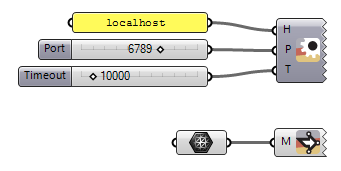
\includegraphics[width=0.47\textwidth]{images/setup03_neu.png}
	\hspace{0.06\textwidth}
	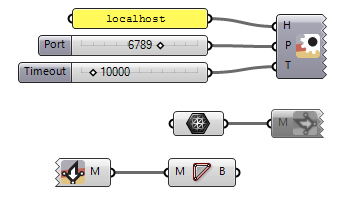
\includegraphics[width=0.47\textwidth]{images/setup04_neu.png}
	\caption{Grasshopper networks connecting Rhino and
          \VaryLab{}. In the first step we send mesh data to \VaryLab{}
          running on the same machine at {\tt localhost:6789}
          (left). In the second step we collect the result from this
          \VaryLab{} instance and create polygons from the mesh's
          faces (right).}
	\label{fig:grasshopper}
\end{figure}

\subfilebibliography

\end{document}

%%% Local Variables: 
%%% mode: latex
%%% TeX-master: "article"
%%% End: 
